\documentclass{article}
\usepackage{graphicx}
\usepackage{color}
\usepackage{url}
\usepackage[font=small,labelfont=bf]{caption}



\begin{document}

\begin{titlepage}
    \begin{center}
        
	\begin{figure}
		\centering
        FACULTY OF MECHANICAL ENGINEERING AND ROBOTICS\\
        AGH UNIVERSITY OF SCIENCE AND TECHNOLOGY\\
        \vspace{0.2cm}
    	\begin{minipage}[b]{0.4\textwidth}
    	    \centering
    		
\includegraphics[width=\textwidth]{IMG/AGH.png}
    	\end{minipage}
    	\hfill
    	\begin{minipage}[b]{0.4\textwidth}
	    	\centering
    		
\includegraphics[width=\textwidth]{IMG/WIMIR.png}
		\end{minipage}
		\vspace{1cm}
    \end{figure}

    \Huge \textbf{Project ICARUS}s
        
    \vspace{0.8cm}
    \LARGE 
    \color{red} ONLY FOR AUTHORIZED PERSONNEL
    \color{black}
            
    \vspace{0.8cm}       
    \textbf{Damian Durczok\\Mikołaj Gacek\\Adam Kolusz}        
    \vfill       
    \vspace{0.8cm}    
    03.03.2018
        
    \end{center}
\end{titlepage}

\tableofcontents
\break

\section{State of Art}
A typical mechatronic device encompasses many fields of technological engineering. This includes mechanical engineering, electronics, computer engineering, systems and control engineering. 

To thoroughly design such a system with awareness of all its elements during each step of the process requires the foresight and knowledge of all the components and relations between individual elements. This is the purpose of the state of art - a prerequisite to the initialization of a project. By the end of this section we will have explored existing technologies and solutions to our problem and drawn up a basic model of the mechatronic device.

\subsection{The Problem}
Certain situations that endanger human life benefit from the intervention of a robotic device. However, these robots may be limited in functionality compared to the human counterpart. In cases such as bomb disposal, nuclear power station decommissioning or handling of dangerous substances the dexterity of a human hand is significantly important.

\subsection{The Solution}
The mechanical hand is a device that has been iterated on many times in recent history. Control of such a hand is either by machine or human. For automated tasks, a machine controlled hand is more than sufficient. However, in unpredictable environments human intervention is still necessary.

This is where the idea stems together. A mechanical hand with the full dexterity of its real counterpart controlled in an intuitive way by a human. The control will be based on the idea of mimicking the operators limbs. Pairing this with a strategically placed camera and a virtual reality headset, we have an operator who is fully immersed and in full control of the situation at hand.

\subsection{Mechanical Hand}
Most modern innovations of the mechanical hand are related to the development of prosthetics. BeBionic \cite{bebionic} and Vincent Systems \cite{vincent} among many others have developed such devices that accurately mimic the likeness.

\begin{center}
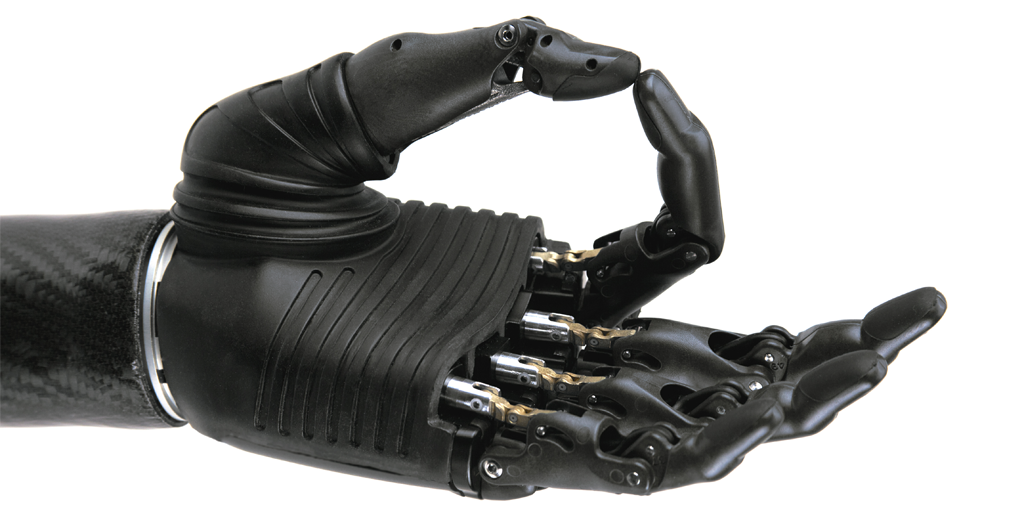
\includegraphics[width=0.5\textwidth]{IMG/Bebionic_V2_Hand.png}
\captionof{figure}{BeBionic Mechanical Hand}
\end{center}

The most popular actuation method is a combination of a DC motor and either a worm gear or lead screw. The size of the hand leaves us with a very small working area, as a result the driving motors must be very small with high gear reductions.

\begin{center}
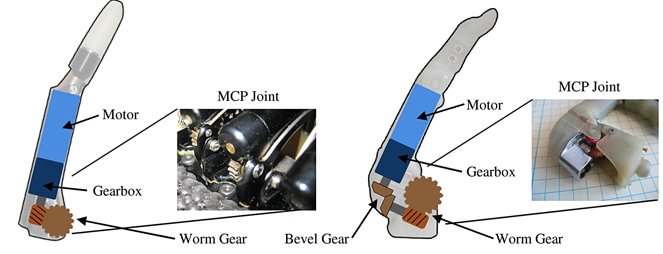
\includegraphics[width=\textwidth]{IMG/fingerMech2.png}
\captionof{figure}{Mechanics of a finger \cite{JRRD}}
\end{center}

Another issue to contend with is the weight and speed of the mechanism. For prosthetic use, the hands are made to be lightweight for mobility. Whereas in our application this isn't a problem, we may still benefit from reducing the moments of inertia by increasing the acceleration capabilities of joints. Ideally having the same dynamic properties as the human hand.\\

The limited working space also forces certain optimizations. For instance, not all joints need to be independently driven. We may simplify the model by involving mechanisms that create a fixed relationship between joints.

\begin{center}
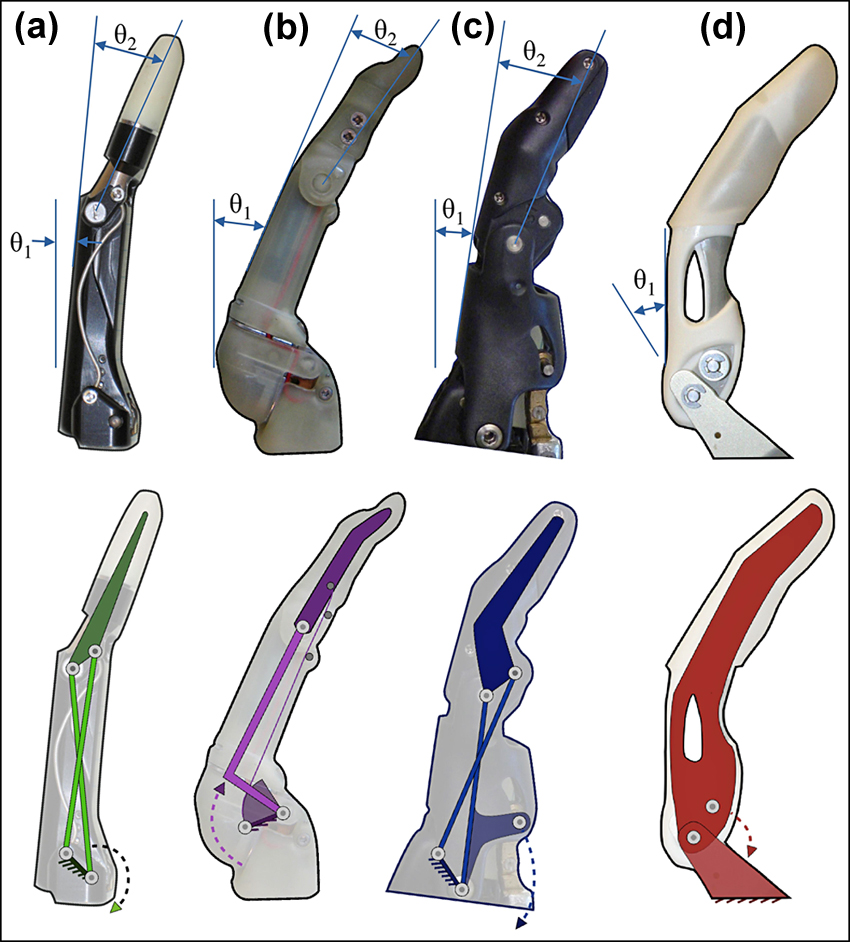
\includegraphics[width=0.5\textwidth]{IMG/fingerMech.jpg}
\captionof{figure}{Reducing degrees of freedom mechanically \cite{JRRD}}
\end{center}

A final feature commonly observed is a certain flexion compliance level. Under a certain level of pressure, the joint flexes by either a spring or flexible material. This is a protective measure to prevent the damage of certain elements.\\

Many hobbyists opt out for a different solution that includes a motor and line. The joints are controlled in one direction by the contraction of a line and in the other by a spring or flexible material. This greatly simplifies the design process by allowing the motors to be located elsewhere. Potentially allowing for much larger drives and a greater gripping force along with greater movement speeds and accelerations. This system also naturally includes flexion compliance.

\begin{center}
\includegraphics[width=0.5\textwidth]{IMG/stringMech.jpg}
\captionof{figure}{Solidworks solution \cite{stringHand}}
\end{center}

This solution isn't as well researched as the earlier method and will require a longer prototyping faze. \\

Pneumatics may offer another solution. All the fingers are actuated by a pneumatic air muscle. These prove to have very high grip strength with favourable dynamic characteristics. All however comes with the price of size, to drive such a system a constant supply of compressed air is necessary to accurately position the stroke-length of each air muscle. Additionally a large valve system is necessary to control such a device.


\begin{center}
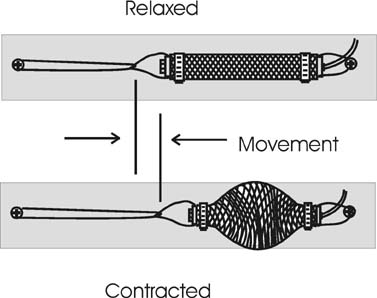
\includegraphics[width=0.4\textwidth]{IMG/airMuscle.jpg}
\captionof{figure}{Air Muscle}
\end{center}
\break
In summary, we may consider driving our mechanism with either an electric motor or a pneumatic device. The pneumatic device may allow for much better dynamic performance such as limb velocity, acceleration and grip strength. However requires an entire pneumatic system in place which may prove expensive and resource heavy. The DC motor compromises on dynamic performance in place for a more ergonomic design.

The driving mechanism may be optimized by involving dependent joints. These joints may be driven directly or at a distance using lines. A line driven mechanism alleviates the problem of having to work in a small working area by removing the largest elements externally. 

\subsection{Control}

\break
\begin{thebibliography}{1}
  \bibitem{bebionic} BeBionic. Retrieved from {\url{http://bebionic.com/the_hand/technical_information/}} 

  \bibitem{vincent} VincentSystems. Retrieved from {\url{  https://vincentsystems.de/en/}} 

  \bibitem{JRRD} U.S. Department of Veterans Affairs, {\em Journal of Rehabilitation Research And Development}. Volume 50 Number 5, 2013
   Pages 599-618 Retrieved form {\url{https://www.rehab.research.va.gov/jour/2013/505/page599.html}}
   
     \bibitem{stringHand} SOLIDWORKS. Retrieved from {\url{ http://blogs.solidworks.com/tech/2016/08/solidworks-time-lapse-tutorial-mechanical-hand.html}} 

     \bibitem{airMuscle} Peter Scarfe, Euan Lindsay {\em Air Muscle Actuated Low Cost Humanoid Hand}. Retrieved from {\url{ http://cdn.intechopen.com/pdfs/4176/InTech-Air_muscle_actuated_low_cost_humanoid_hand.pdf
}} 
\end{thebibliography}
  
\end{document}